\section*{Consigna 2}

Se quiere enviar un paquete de 2000 B de payload desde \textbf{A} hasta \textbf{B} utilizando IPv4 a través de una red cuya topología se muetra a continuación. DF inicial es 0.

\begin{figure}[H]
    \centering
    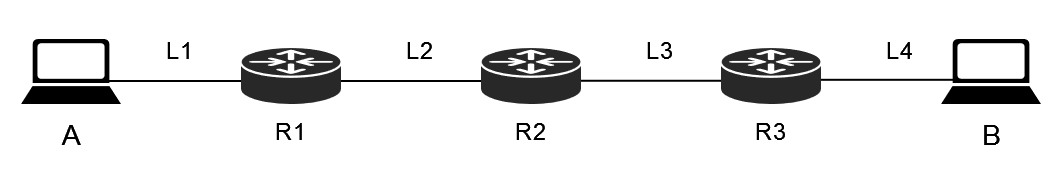
\includegraphics[width=0.9\linewidth]{Images/topologia.png}
\end{figure}

\vspace{-5mm}
{
\renewcommand{\arraystretch}{1.5}
\begin{table}[H]
    \centering
    \begin{tabular}{|c|c|c|c|c|}
    \hline
     & L1 & L2 & L3 & L4 \\ \hline
    MTU (B) & 1700 & 600 & 598 & 560\\ \hline
    \end{tabular}
\end{table}
}


Llenar la siguiente tabla con todos los paquetes que lleguen al host:

\begin{table}[H]
    \centering
    \renewcommand{\arraystretch}{1.5}
    \begin{tabular}{|c|c|crrrrr|}
    \hline
    \multirow{2}{*}{Name} & \multirow{2}{*}{Payload Size} & \multicolumn{6}{c|}{Datagram Header} \\ \cline{3-8} 
     &  & \multicolumn{1}{c|}{IHL} & \multicolumn{1}{c|}{Total Length} & \multicolumn{1}{c|}{ID} & \multicolumn{1}{c|}{MF} & \multicolumn{1}{c|}{DF} & \multicolumn{1}{c|}{Fragment Offset} \\ \hline
    \multicolumn{1}{|r|}{} & \multicolumn{1}{r|}{} & \multicolumn{1}{r|}{} & \multicolumn{1}{r|}{} & \multicolumn{1}{r|}{} & \multicolumn{1}{r|}{} & \multicolumn{1}{r|}{} &  \\ \hline
    \multicolumn{1}{|r|}{} & \multicolumn{1}{r|}{} & \multicolumn{1}{r|}{} & \multicolumn{1}{r|}{} & \multicolumn{1}{r|}{} & \multicolumn{1}{r|}{} & \multicolumn{1}{r|}{} &  \\ \hline
    \end{tabular}
\end{table}

